\chapter{Introducción}
\label{chap1}
\chapterquote
%~ {Don't get involved in partial problems, 
%~ but always take flight to where there is a free view over the whole single great problem, 
%~ even if this view is still not a clear one.}
{No se involucre en problemas parciales,
siempre tome vuelo hacia donde hay una vista libre sobre el gran problema único,
incluso cuando esta visión todavía no sea clara.}
{Ludwig Wittgenstein, 1889-1951}

\section{Motivación}
\label{1:motivacion}

La creciente sofisticación en los análisis de ingeniería demanda el estudio de sistemas cada vez más complejos.
Un ejemplo actual de esto es el modelado de grandes componentes termohidráulicos de geometría muy compleja en la industria nuclear. 
Es notable la presencia de subsistemas de caracterísiticas muy diferentes: principalmente diferentes tamaños y regímenes de flujos. 
Si bien se necesita modelar y entender el sistema completo, solo es de interés el detalle en algunos subsistemas. 
Algunos, como las tuberías, se hallan muy bien caracterizados por modelos simple (ODE's).
Otros, en cambio, requieren un análisis detallado de flujo, y por ello es necesaria la simulación fluidodinámica computacional (CFD).

En este marco se justifica el desarrollo de una técnica numérica que permita desglosar problemas complejos 
en subsistemas que puedan ser analizados por separado mediante condiciones de borde dinámicas.
Como referencia a este enfoque se citan los trabajos desarrollados por J. S. Leiva y G. C. Buscaglia (2006) \cite{coup-0d3d}, P.J. Blanco et al. (2010) \cite{coup-black} y J. S. Leiva et al. (2011) \cite{coup-hyd}.

\section{Abordaje del modelado}
\label{1:abordaje}

\subsection*{Desglosado del sistema original en subsistemas acoplados}
\label{1:acoplamiento}

Dado un sistema $S$ en un dominio $\Omega$ con borde $\Gamma$, es posible desglosar este dominio en $N$ particiones 
y analizar diferentes subsistemas $S_i,i=1,...,N$ por separado, acoplados entre sí mediante condiciones de borde en las uniones
(Método de Descomposición Disjunta de Dominios \cite{ddmethod}).
Las condiciones de borde originales del problema, impuestas sobre la curva $\Gamma$,
ahora se imponen sobre cada fragmento de la curva.
La Figura \ref{esquema-acoplamiento} presenta el esquema propuesto.
La notación utilizada es la siguiente:
\begin{itemize}
\item $S_i$ representa al subsistema $i$, $i=1,...,N$.
\item $U_{i,j}^k$ es la unión $k$ entre subsistemas $i$ y $j$, $k=1,...,K_{i,j}$.
\item $I_{S_i}^{l}$ es la interfaz local $l$ del subsistema $S_i$, $l=1,...,L_i$.
\item $\Gamma_i$ es la porción de frontera exterior en el subsistema $N$,
 $\Gamma_1$ $\cup$ $\Gamma_2$ $\cup$ ... $\cup$ $\Gamma_i$ ...  $\cup$ $\Gamma_N$ = $\Gamma$.
 Notar que $\Gamma_j$ puede ser nula para algún $S_j$.
\item ${(x_m)_{S_i}^{I_l}}$ es el valor de la variable $x_m$ en la interfaz ${I_l}$ del subsistema ${S_i}$, $m=1,...,M_i$.
\item ${(\bar{x})_{S_i}^{I_l}}$ es el vector de incógnitas $\{x_1,x_2,...,x_{M_i}\}$ en la interfaz ${l}$ del subsistema ${i}$.
\end{itemize}

\begin{figure}[ht]
\centering{}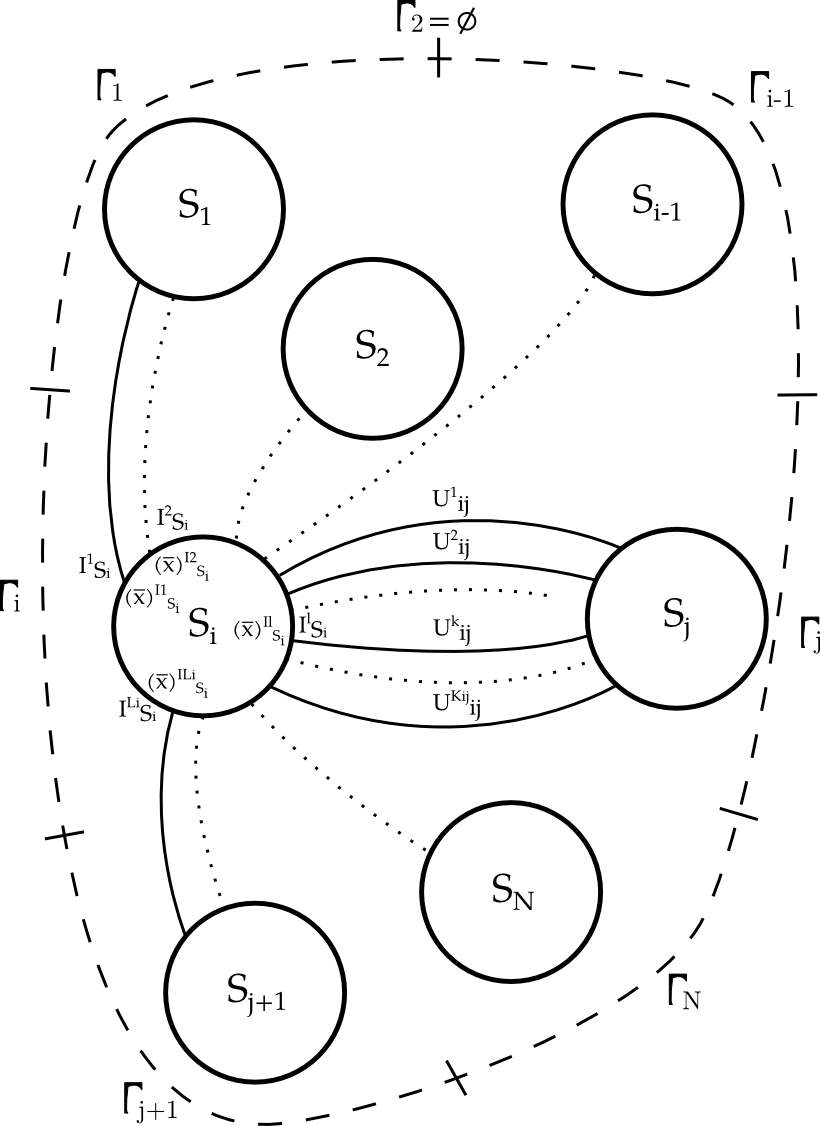
\includegraphics[scale = 0.4]{coupling_systems.png}
\caption[Esquema de sistema complejo analizado mediante el Método de Descomposición Disjunta de Dominios]
{Esquema de sistema complejo analizado mediante el Método de Descomposición Disjunta de Dominios.} 
\label{esquema-acoplamiento} 
\end{figure}
La idea ahora es resolver los subsistemas por separado, pero en principio esto no es posible porque las condiciones de borde de las interfaces de acople son desconocidas.
Es decis, existen tantas incógnitas como variables en cada interfaz.
Sin embargo, es posible notar que la unión $U_{i,j}^k$ que relaciona los sistemas $S_{i}$ y $S_{j}$ 
mediante las interfaces $I_{S_{i}}^{l_1}$ e $I_{S_{j}}^{l_2}$ respectivamente, 
define una relación de continuidad\footnote{
Las incógnitas que representan derivadas normales en la interfaz de acople pueden tomar signos opuestos según la convención.
Por ejemplo, si el flujo de calor es una incógnita, 
y se define como flujo positivo a aquel que es saliente del subsistema, 
entonces la condición de continuidad implicará que:
\begin{equation*}
{(q")_{S_i}^{I_{l_1}}}=-{(q")_{S_j}^{I_{l_2}}}
\label{continuidad-q}
\end{equation*}
} entre las incógnitas ${(x_m)_{S_i}^{I_{l_1}}}$ y ${(x_m)_{S_j}^{I_{l_2}}}$, de tal forma que:

\begin{equation}
{(x_m)_{S_i}^{I_{l_1}}}={(x_m)_{S_j}^{I_{l_2}}}
\label{continuidad}
\end{equation}
Estas relaciones reducen a la mitad la cantidad de incógnitas.
Las demás ecuaciones necesarias para despejar las incógnitas se encuentran a partir del modelo de estudio de cada subsistema. 
Sean $(\mathscr{F}_m)_{i}^{l}$ las relaciones funcionales que calculan el valor de las incógnitas ${(x_m)_{S_i}^{I_l}}$ en la interfaz $l$ del subsistema $i$,
a partir del valor de otras incógnitas y de los datos de contorno sobre la frontera exterior $\Gamma_i$.
Se tiene que:

\begin{equation}
\begin{split}
  (x_m)_{S_i}^{I_l} = (\mathscr{F}_m)_{i}^{l} \left ( (\bar{x})_{S_i}^{I_1}, (\bar{x})_{S_i}^{I_2}, ..., 
  (\bar{x})_{S_i}^{I_{L_i}}, (\alpha_i({\Gamma_i}) \right )
\end{split}
\label{ecuaciones-modelos}
\end{equation}
donde $(\alpha_i({\Gamma_i})$ representa las condiciones de borde impuestas sobre la curva $\Gamma_i$.
Estas relaciones $(\mathscr{F}_m)_{i}^{l}$, básicamente, mapean condiciones de borde de un tipo, que son impuestas como datos, en condiciones de borde de otro tipo.
Notar que algunas de las dependencias pueden anularse dependiendo del modelo de estudio utilizado en cada subsistema.
Cuando la expresión \ref{ecuaciones-modelos} es más sencilla y solo involucra el valor de otro tipo de condición de borde para la misma interfaz,
la relación funcional recibe el nombre de operador \textit{Steklov-Poincaré}\footnote{
En matemática, el operador \textit{Steklov-Poincaré} mapea el valor de una condición de borde de una PDE elíptica en un dominio al valor
de otra condición de borde (por ejemplo, una condición de borde de tipo \textit{Dirichlet} en una condición de borde de tipo \textit{Neumann}).
Usualmente, cualquiera de las dos condiciones determinan la solución.
}.
Considerando estas ecuaciones, el problema general abordado mediante el Método de Descomposición Disjunta de Dominios queda bien definido.

\subsection*{Estrategia de resolución del acoplamiento}
\label{1:ecuaciones}
Una vez planteadas las ecuaciones del problema, es necesario definir una estrategia de resolución.
A continuación se propone un ejemplo didáctico para comprender las estrategias de acoplamiento posteriormente cometadas.

\medskip

\begin{EvalBox}{\textbf{Ejemplo:} Cálculo de temperaturas con el Método de Descomposición Disjunta de Dominios}

Se desea resolver un problema de cálculo de campo de temperatura mediante el Método de Descomposición Disjunta de Dominios.
El sistema global de análisis es una barra unidimensional de longitud $L$ con condiciones de borde homogéneas, fuente interna de energía $f$ y conductividad térmica $k$.
El modelo matemático utilizado es el siguiente:
\begin{equation}
\left\{\begin{matrix}
-k \Delta u=f \\
\left.u\right|_{\partial\Omega}=0
\end{matrix}\right.
\label{ecuacion-calor}
\end{equation}
Resolver el problema particionando el dominio original $[0,L]$ en los subdominios $[0,c]$ y $[c,L]$ como se muestra en la Figura \ref{temp-ej}:
    
  \centering
  \begin{tikzpicture}
	\node at (12.5,4em) (om) {$\Omega$};

	\node at (7.5,5.9em) (Olabel) {0}; % 0
	\node at (7.5,5em) (O) {}; % point 0

	\node at (14.5,6.9em) (clabel) {c}; % c
	\node at (14.5,5em) (c) {}; % point c

	\node at (17.5,5.9em) (llabel) {L}; % L
	\node at (17.5,5em) (l) {}; % point L

	\draw[line width=1pt, o-|] (O) -- (c.center); % primer extremo de barra completa
	\draw[line width=1pt, |-o] (c.center) -- (l); % segundo extremo de barra completa

	\draw[line width=0.8pt,->] (11,3.5em) -- (10,1.5em); % primer flecha
	\draw[line width=0.8pt,->] (16,3.5em) -- (17,1.5em); % segunda flecha

	\node at (10,-1em) (om1) {$\Omega_1$};
	\node at (6.5,0.9em) (O1label) {0};
	\node at (6.5,0em) (O1) {};
	\node at (13.5,0.9em) (c1label) {c};
	\node at (13.5,0em) (c1) {};

	\draw[line width=1pt, o-o] (O1) -- (c1); % primer barra

	\node at (17,-1em) (om2) {$\Omega_2$};
	\node at (15.5,0.9em) (c2label) {c};
	\node at (15.5,0em) (c2) {};
	\node at (18.5,0.9em) (l2label) {L};
	\node at (18.5,0em) (l2) {};

	\draw[line width=1pt, o-o] (c2) -- (l2); % segunda barra
  \end{tikzpicture}
  \captionof{figure}
  [Descomposición disjunta de dominios en el cálculo del campo de temperatura a lo largo de una barra unidimensional]
  {Descomposición disjunta de dominios en el cálculo del campo de temperatura a lo largo de una barra unidimensional.}
  \label{temp-ej}
  
\end{EvalBox}

El método consiste en la resolución de \ref{ecuacion-calor} en cada subdominio,
pero la condición de borde en $\partial \Omega$ ahora aplica solo sobre el borde original del dominio.
Para que cada problema quede bien planteado es necesario imponer una condición de borde extra en el punto de acople $c$ de cada subsistema.
Esta decisión depende de la estrategia empleada para resolver el acoplamiento.

La forma clásica de resolución es el método \textit{Dirichlet-to-Neumann}.
Este método es un método explícito de simple implementación, que resuelve el acoplamiento mediante iteraciones de tipo \textit{Picard}.
En el método \textit{Dirichlet-to-Neumann}, es necesario decidir qué subsistema va a ser resuelto en primera instancia,
y qué tipo de condición de borde se le va a aplicar.
Estas primeras decisiones son arbitrarias.
En la resolución del ejemplo se decide comenzar con el subsistema de la izquierda e
imponer una temperatura $(T_{guess})_{S_1}$ (condición \textit{Dirichlet}) en su interfaz de acople.
Luego de realizar el cálculo de temperaturas queda definido un flujo de calor a través de esta interfaz.
Es decir, uno de los valores de las incógnitas en la interfaz de acople se calcula como función del valor de la otra incógnita, 
que fue supuesta como dato, a partir de la relación \ref{ecuaciones-modelos}.
En este caso la relación recibe el nombre de operador \textit{Steklov-Poincaré} y se define como:
\begin{equation}
(q''_{calc})_{S_1} = \mathscr{N}_1\left ((T_{guess})_{S_1}\right )
\label{q_n_t}
\end{equation}
donde $\mathscr{N}$ es el operador que mapea condiciones de borde de tipo \textit{Dirichlet} en condiciones de borde de tipo \textit{Neumann}
y $(q''_{calc})_{S_1}$ es el flujo de calor calculado.
En base a la relación de continuidad \ref{continuidad} este flujo de calor se impone en el segundo subsistema como condición de borde.
Esta condición define nuevamente una temperatura $(T_{calc})_{S_2}$ en la interfaz de acople, mediante el operador \textit{Steklov-Poincaré} definido en este subdominio:
\begin{equation}
(T_{calc})_{S_2} = \mathscr{D}_2\left ((q''_{calc})_{S_1}\right )
\label{t_d_q}
\end{equation}
donde $\mathscr{D}$ es el operador que mapea condiciones de borde de tipo \textit{Neumann} en condiciones de borde de tipo \textit{Dirichlet}.
Si $(T_{calc})_{S_2}$ coincide con $(T_{guess})_{S_1}$ inicialmente supuesta,
los resultados están convergidos y entonces finaliza el cálculo
En caso contrario, el proceso debe repetirse, pero ahora se impone $(T_{calc})_{S_2}$ al primer subsistema.
El cálculo continúa así hasta que los valores $\{(q''_{calc})_{S_1}, (T_{calc})_{S_2}\}$ convergen en iteraciones contiguas.

Si inicialmente se hubiera impuesto una condición de tipo \textit{Neumann} en el primer subdominio, 
necesariamente al segundo subdominio debería habérsele impuesto una condición de tipo \textit{Dirichlet},
ya que la variable calculada en la interfaz de acople por el primer subsistema hubiera sido una temperatura.
Es decir, al utilizar el método \textit{Dirichlet-to-Neumann}, la elección de un tipo de frontera en un subdominio dado determina el tipo de frontera en el subdominio contiguo,
para las ecuaciones que relacionan las mismas variables de estado en ambos subsistemas (aquí solo existe una única variable de estado, la temperatura).
Esta característica es un poco restrictiva, ya que no permitiría, por ejemplo, que todos los subproblemas de análisis se resuelvan con condiciones de borde de tipo \textit{Dirichlet}.

Sin embargo esta no es la única desventaja del método \textit{Dirichlet-to-Neumann}.
Otra desventaja es que en general requiere demasiadas iteraciones para converger \cite{fede-enief2016}.
En algunos problemas el método puede quedar estancado, iterando en series de valores que se repiten en ciclo.
Y en otros casos el método es divergente (sin ir más allá, para un cierto conjunto de parámetros del problema ejemplo analizado, el método diverge, ver \cite{coup-strong}).

Existe una forma alternativa de resolver el acoplamiento.%, y es mediante una técnica implícita.
Esta técnica es una metodología también iterativa, y consiste en la evaluación de residuos sucesivos construidos por diferencia entre valores propuestos y valores calculados.
En primera instancia se propone un valor \textit{guess} para todas las incógnitas $(x_{m}^{guess})_{S_i}^{I_l}$.
Estos valores deben respetar las relaciones de continuidad \ref{continuidad}.
En segunda instancia se decide qué tipos de condiciones de borde va a recibir cada interfaz de cada subsistema,
definiendo problemas parciales bien planteados.
En el ejemplo analizado, sería posible definir condiciones de borde de tipo \textit{Dirichlet} en ambos subsistemas.
En función de esta decisión, se toman los valores correspondientes del vector $\bar{x}_{guess}$ y se establecen como datos para cada problema parcial.
Una vez resuelto el problema en cada subdominio, se calcula el valor de las variables que no fueron tomadas como dato en las interfaces de acople.
En el ejemplo, si se había establecido un valor de temperatura como condición de borde de tipo \textit{Dirichlet} en ambas interfaces,
se calcula entonces el valor del flujo de calor en la misma interfaz para cada subsistema, mediante los operadores de \textit{Steklov-Poincaré} $\mathscr{N}_1$ y $\mathscr{N}_2$:
\begin{equation}
\left\{\begin{matrix}
(q''_{calc})_{S_1}  = \mathscr{N}_1\left ((T^{guess})_{S_1}\right ) \\
(q''_{calc})_{S_2}  = \mathscr{N}_2\left ((T^{guess})_{S_2}\right )
\end{matrix}\right.
\label{qq_nn_tt}
\end{equation}

Al hacer esto se están resolviendo las ecuaciones \ref{ecuaciones-modelos},
obteniéndose los valores $(x_{m}^{calc})_{S_i}^{I_l}$.
Finalmente, se computan las diferencias entre los valores \textit{guess} y los valores calculados, obteniendo los residuos $(r_m)_{i}^{l}$:

\begin{equation}
(r_m)_{i}^{l} = (x_{m}^{guess})_{S_i}^{I_l} - (x_{m}^{calc})_{S_i}^{I_l}
\label{ecuaciones-residuos}
\end{equation}
donde $m$ es el índice de incógnita, $l$ de la intefaz e $i$ del subsistema.
En el ejemplo, las ecuaciones de residuos quedarían:
\begin{equation}
\left\{\begin{matrix}
(r_{q''})_{S1}^{1}  = (q''^{ guess})_{S_1} - (q''^{calc})_{S_1} \\
(r_{q''})_{S2}^{1}  = (q''^{ guess})_{S_2} - (q''^{calc})_{S_2}
\end{matrix}\right.
\label{res_qq}
\end{equation}

La convergencia fuerte de los subsistemas acoplados requiere que estos residuos sean nulos, y por lo tanto se busca el siguiente resultado:
\begin{equation}
\bar{r}(\bar{x}^{guess})=\bar{0}
\label{sistema-simple}
\end{equation}
donde $\bar{r}$ es el vector de residuos de las ecuaciones,
y $\bar{x}^{guess}$ es el vector que contiene los valores $(x_m^{guess})_{S_i}^{I_l}$ propuestos.
Comúnmente en la primera iteración esto no sucede, y por lo tanto es necesario repetir el proceso sucesivas veces hasta obtener convergencia.
En la siguiente sección se comentan diferentes métodos numéricos para la resolución del sistema de ecuaciones \ref{sistema-simple}.

\subsection*{Métodos numéricos para la resolución de sistemas de ecuaciones de residuos}
\label{1:metodos}

Existen diferentes métodos numéricos para hallar las raíces del sistema de ecuaciones \ref{sistema-simple}.
El método más básico es el método del punto fijo, que es un método iterativo explícito\footnote{
Puede pensarse a este método como una combinación de múltiples métodos \textit{Dirichlet-to-Neumann} efectuados al mismo tiempo,
en el que en cada iteración se realiza el cálculo en cada subdominio a partir de los resultados obtenidos en otros subdominios en la iteración previa.
},
y consiste en tomar como semilla $\bar{x}^{guess}_n$ para cada iteración $n$ al resultado $\bar{x}^{calc}_{n-1}$ de la iteración previa.
Este método, al igual que el método \textit{Dirichlet-to-Neumann}, tiene bajo orden de convergencia,
y tampoco permite combinar libremente la elección de condiciones de borde para los diferentes subdominios.

Los métodos más eficientes para la resolución de sistemas de ecuaciones de residuos son métodos implícitos,
en los que la semilla para cada iteración no es directamente el resultado obtenido en la iteración previa.
De ahora en adelante para simplificar la notación se usa $\bar{x}_n$ en lugar de $\bar{x}^{guess}_n$.
Haciendo un desarrollo de Taylor de las ecuaciones de residuos alrededor del punto $\bar{x}_n$, 
truncando los términos superiores al primer orden, y evaluando en $\bar{x}=\bar{x}_{n+1}$ se tiene:

\begin{equation}
\bar{r}(\bar{x}_{n+1}) = \bar{r}(\bar{x}_n) + \nabla \bar{r}(\bar{x}_n)(\bar{x}_{n+1}-\bar{x}_n)
\label{taylor}
\end{equation}
donde $\nabla \bar{r}(\bar{x}_n)$ es la matriz jacobiana del sistema $\mathbb{J}$ evaluada en el punto $\bar{x}_n$, 
cuyo elemento $J_{ij}$ debe evaluarse como $J_{ij}=\frac{\partial r_i}{\partial x_j}$.
Suponiendo que ${\bar{x}_{n+1}}$ tiende a la raíz buscada se ha de cumplir que $\bar{r}(\bar{x}_{n+1})=0$.
Sustituyendo en \ref{taylor} y operando algebraicamente se llega a la siguiente expresión:

\begin{equation}
\bar{r}(\bar{x}_n) = -\mathbb{J}(\bar{x}_n)(\bar{x}_{n+1}-\bar{x}_n)
\end{equation}
Para hallar la solución $\bar{x}_{n+1}$ simplemente hay que resolver el sistema:

\begin{equation}
\bar{x}_{n+1} = \bar{x}_{n} -\mathbb{J}^{-1}(\bar{x}_n)\bar{r}(\bar{x}_n)
\end{equation}
que es el método de iterativo \textit{Newton-Raphson}.
La principal ventaja de este método es que tiene orden de convergencia cuadrática,
pero la desventaja es que para utilizar este método se requiere la construcción de la matriz jacobiana en cada iteración, lo cual es demasiado costoso.
Una sencilla aproximación mediante diferencias finitas de primer orden de cada elemento de la matriz jacobiana requiere numerosas evaluaciones.
Cada elemento $J_{ij}=\frac{\partial R_i}{\partial x_j}$ puede aproximarse mediante diferencias finitas a primer orden como:
\begin{equation}
J_{ij} \approx \frac{r_i(\bar{x}_j + \Delta \bar{x}_j) - r_i(\bar{x}_j)}{\left\|\Delta x_j\right\|}
\label{j-diff}
\end{equation}
donde $\Delta \bar{x}_j$ es un vector que contiene valores nulos en todos sus elementos excepto en el elemento de la posición $j$,
cuyo valor es la diferencia incremental para la variable $j$.
La construcción de la matriz jacobiana con éste método requiere una evaluación del vector residuo $\bar{r}$ en el punto $\bar{x}$ y luego $N_{unk}$ evaluaciones extras,
donde $N_{unk}$ es la cantidad total  de incógnitas. 
Es decir, en total, se requieren $N_{unk}+1$ evaluaciones.
Si bien estas evaluaciones son independientes entre sí y por lo tanto altamente paralelizables, este método requiere excesivos recursos de cálculo.

Una forma alternativa y elegante de resolver el sistema de ecuaciones planteado en \ref{sistema-simple} es mediante métodos \textit{quasi-Newton}.
La característica principal de estos métodos es que aproximan la matriz jacobiana sin necesidad de realizar evaluaciones extras en todas las iteraciones,
y por lo tanto tienen una ventaja fuerte frente al método de \textit{Newton-Raphson}.
Además, en general tienen mayor orden de convergencia que los métodos mediante iteraciones de \textit{Picard}.

El método de \textit{Broyden} es uno de estos métodos \cite{broyden}.
La matriz jacobiana $\mathbb{B}_n$ en la iteración $n$ es aproximada mediante una matriz $\mathbb{B}_n$ que se construye solo en función 
del valor de los vectores incógnitas $\bar{x}_{n-1}$ y $\bar{x}_{n}$,
de los vectores residuos $\bar{r}_{n-1}$ y $\bar{r}_{n}$,
y de la matriz de la iteración previa $\mathbb{B}_{n-1}$:
\begin{equation}
\mathbb{B}_n = \mathbb{B}_{n-1} + \frac{\Delta{\bar{r}_n}-\mathbb{B}_{n-1}\Delta{\bar{x}_n}}{\left \| \Delta{\bar{x}_n} \right \| ^2}\Delta{\bar{x}}_n^T
\label{broyden}
\end{equation}
donde $\Delta{\bar{r}_n}=\bar{r}_n - \bar{r}_{n-1}$ y $\Delta{\bar{x}_n}=x_n - \bar{x}_{n-1}$.
Existe una variante del método, el método \textit{Broyden ortonormal} \cite{broyden-on}, que aproxima la matriz $\mathbb{B}_n$ en función de una base vectorial de residuos previos calculados.
Este método asegura la convergencia en una cantidad finita de iteraciones para sistemas lineales, (la cantidad de iteraciones requerida es la dimensión de la matriz jacobiana).
Ambos métodos tienen convergencia superlineal \cite{kelley}.

Otro métodos \textit{quasi-Newton} muy utilizados son el método de la secante (\textit{chord method}) \cite{kelley} y el método de \textit{Shamanskii} de tipo $m$.
El primero calcula la matriz jacobiana solo en la primer iteración y la utiliza sin actualizaciones en el resto de las iteraciones.
El segundo también calcula la matriz jacobiana en la primer iteración, y vuelve a calcularla cada $m$ iteraciones.
Este método también tiene convergencia superlineal \cite{kelley}.

Existe también un conjunto de métodos conocidos como métodos \textit{Newton-Krylov} \cite{kelley} para la resolución del sistema \ref{sistema-simple}.
Estos métodos no requieren el cálculo de matriz jacobiana (\textit{matrix-free methods}).
Sin embargo, en cada paso de iteración de resolución del sistema no lineal (\textit{outer iteration}) requieren múltiples iteraciones del método de \textit{Krylov} (\textit{inner iterations}),
y en cada una de ellas calculan variaciones en las direcciones de descenso seleccionadas,
lo cual implica múltiples evaluaciones de funciones.
Por este motivo estos métodos resultan altamente costosos.

En la resolución de sistemas de ecuaciones no lineales mediante cualquiera de los métodos imlpícitos
puede utilizarse una técnica de aceleración conocida en la bibliografía como \textit{line searching} \cite{kelley}. 
Esta técnica consiste en búsquedas del mínimo a lo largo de la última dirección de cambio en cada iteración, empleando evaluaciones de funciones extras.

\subsection*{Problemas de evolución}
\label{1:evolucion}
En problemas de evolución la estrategia es permitir que cada subsistema avance por separado acoplando sus resultados mediante las ecuaciones \ref{sistema-simple} solo cada ciertos pasos.
Esto se permite porque cada subsistema podría requerir subpasos de evolución diferentes\footnote{
Distintos subdominios pueden tener diferentes requisitos sobre el parámetro de evolución, dependiendo de la física implicada.
Algunos, por ejemplo, podrían experimentar transitorios fluidodinámicos, en los que es de interés mantener por debajo de algún valor 
ciertos parámetros numéricos (como el número de \textit{Courant}) proporcionales al paso de tiempo.
Otros, en cambio, podrían estar siendo resueltos mediante métodos complejos que consumieran elevados recursos temporales,
por tanto sería de interés utilizar subpasos evolutivos mayores.
}. Notar que no es necesario mantener la misma estrategia de selección de condiciones de borde para cada interfaz a lo largo de la evolución.
Las variables que son datos o incógnitas para cada subdominio pueden irse alternando,
seleccionando diferentes ecuaciones \ref{ecuaciones-modelos} a resolver en diferentes pasos de acople.
Debido a la convergencia fuerte de los valores de las variables en las interfaces de acople,
el método es incondicionalmente estable a lo largo de la evolución.

\section{Objetivos y estructura de trabajo}
\label{1:objetivos}
Considerando la motivación y la formulación precedente, queda establecido el siguiente objetivo general de la maestría:

\vspace{1em}
\begin{addmargin}[1.5em]{1.5em}
\textit{Desarrollar una estrategia de resolución de problemas complejos formulados mediante el
Método de Descomposición Disjunta de Dominios que permita resolver subproblemas separados con códigos de cálculo específicos,
manteniendo la interacción entre ellos solo mediante condiciones de borde.}
\end{addmargin}
\vspace{1em}

La estructura de la tesis es detallada a continuación.
En el presente \hyperlink{chapter.1}{capítulo} se han planteado las ecuaciones que surgen al plantear problemas complejos mediante el Método de Descomposición Disjunta de Dominios,
y se han presentado alternativas numéricas para la resolución de las mismas.
En el \hyperlink{chapter.2}{Capítulo 2} se describe la estrategia para la resolución de problemas acoplados mediante diferentes programas de cálculo.
Se presenta la estructura de comunicación definida y se describen las implementaciones necesarias para su funcionamiento.
En el \hyperlink{chapter.3}{Capítulo 3} se muestran algunas aplicaciones de la herramienta estudiada.
La primera aplicación es un sistema fluídico cerrado gobernado por fuerzas naturales, que se estudia subdividiéndolo en dos subsistemas, con dos interfaces de acople cada uno.
El siguiente sistema de estudio es el vaciado del tanque reflector de un reactor de investigación.
Interesa analizar el tiempo de descarga ya que el mismo es diseñado como sistema de seguridad.
Se abordan distintos modelos multiescala del mismo, para estudiar el detalle fluídico tridimensional en un componente del sistema,
acoplando con condiciones de borde dinámicas a un modelo cero-dimensional que representa el resto del sistema.
El tercer sistema de análisis es un modelo de redes hidráulicas con múltiples componentes.
Con este estudio se busca demostrar la eficiencia de la herramienta en acoples fluidodinámicos de mayor escala.
Sobre el final del capítulo se extiende la herramienta a problemas multifísicos que engloban el acoplamiento fuerte de múltiples fenómenos.
Se analizan dos ejemplos de acoplamiento neutrónico-termohidráulico.

